% SPDX-FileCopyrightText: 2025 Jorge Teixeira Crespo <jorge.teixeira@udc.es>
%
% SPDX-License-Identifier: GPL-2.0-or-later

\chapter{Project Methodology}
\label{chap:project-methodology}

\lettrine{T}{ransparency}, reproducibility, and effective collaboration through open tools and platforms form the foundation of this thesis's development methodology. Given the diverse schedules and availability constraints of those involved, asynchronous communication has been explicitly chosen as the primary mode of interaction. This approach facilitates flexibility, allows thorough peer review, and accommodates the varying responsibilities of project participants.

\section{Open Development}

The entire thesis development is conducted openly within a public GitHub repository.\footnote{\url{https://github.com/jorgeteixe/thesis}} All thesis source files, configurations, and relevant documentation are version-controlled, publicly accessible, and managed using a pull request workflow. This enables structured peer review of both technical decisions and thesis content. Continuous integration is automated through GitHub Actions, which generate the thesis PDF document upon every change. This approach ensures immediate feedback, reproducibility, and simplifies collaboration with supervisors.

Throughout the thesis, all configurations, scripts, and tools subject to being open-sourced are either already publicly available or will be made publicly available.\footnote{\url{https://github.com/gpul-org}} Official documentation will be openly hosted on the association's website, providing comprehensive guidance and ensuring traceability and accountability for all project-related decisions. This open and documented approach not only supports transparency but also creates a valuable resource for future students, contributors, and maintainers.

\section{Planning and Methodology}

\lettrine{T}{he} planning for this thesis follows a structured approach inspired by the classic \emph{Waterfall} methodology. This choice is primarily driven by the clear and sequential dependencies between project phases, which naturally fit a linear model.

The initial planning stage involves a comprehensive forensic analysis of the existing infrastructure, clearly identifying active services, their usage, and existing limitations. The subsequent phase, state-of-the-art analysis, builds directly upon this initial assessment. Each required service is systematically evaluated through practical testing, informing both technological decisions and preliminary resource estimates.

In parallel, potential hosting providers are to be explored. Although initial resource requirements can be estimated after evaluating candidate technologies, final confirmation depends on the definitive technology selection, establishing a clear dependency between these tasks.

Implementation is planned to proceed sequentially due to explicit task dependencies: setting up the hosting provider account, installing the base system, configuring container environments, and deploying selected services in a predetermined order. Documentation and thesis writing activities will run concurrently to ensure comprehensive records of the processes.

Finally, a structured migration and handover phase is planned after thesis submission. This phase will ensure operational readiness and facilitate effective knowledge transfer to future maintainers, reinforcing sustainability.

A Gantt chart illustrating these phases is shown in Figure~\ref{fig:gantt-planned}, spanning a four-month period from March 1st to the beginning of July.

\begin{figure}[H]
  \centering
  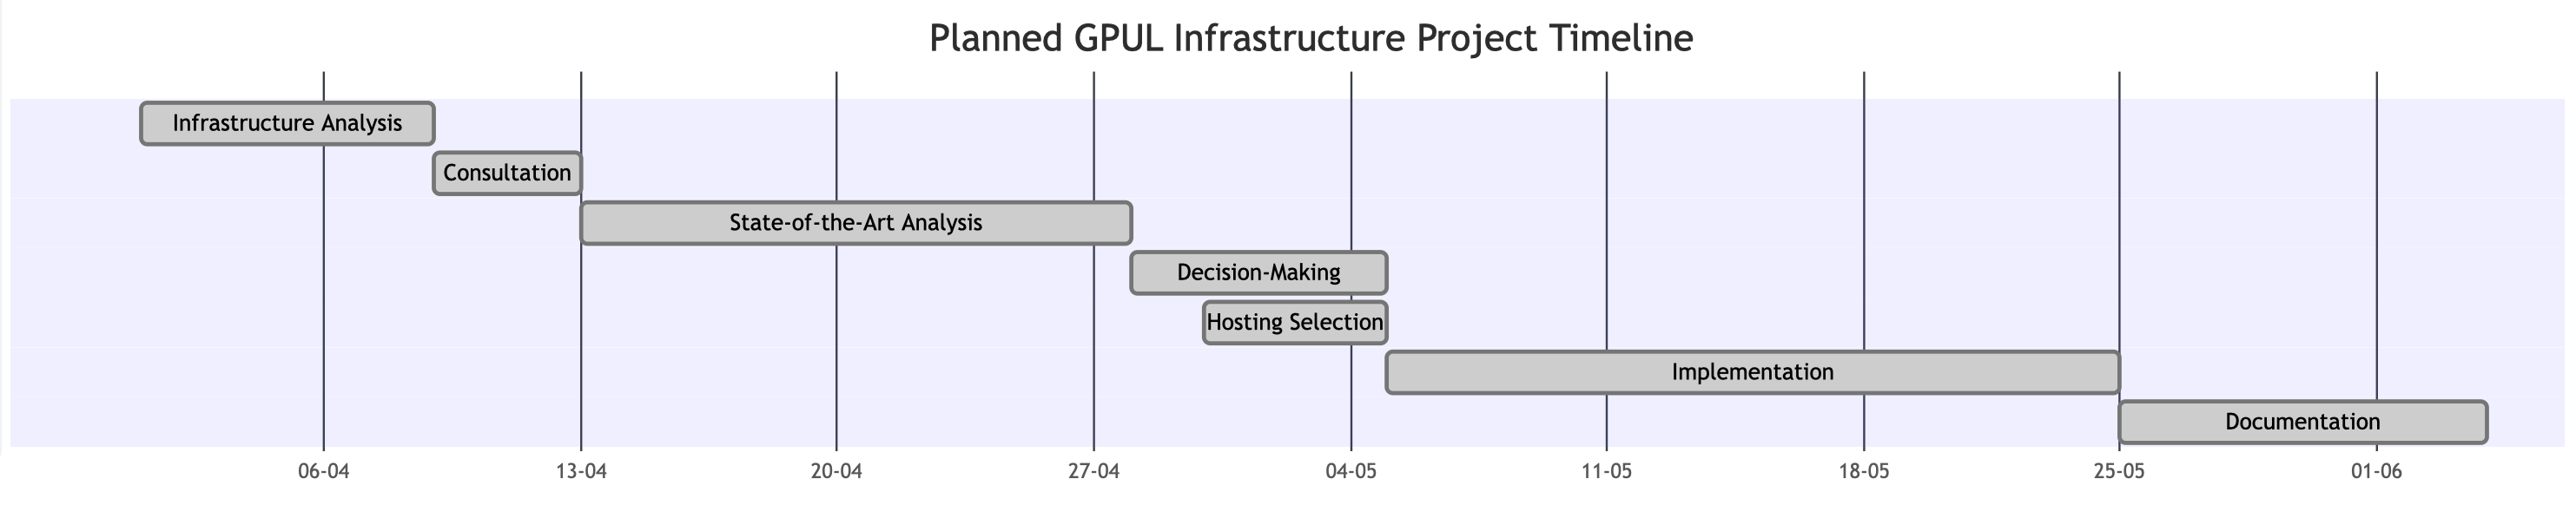
\includegraphics[width=1\textwidth]{imaxes/gantt-planned.png}
  \caption{Gantt chart illustrating the planned project phases.}
  \label{fig:gantt-planned}
\end{figure}

\subsection*{Phases}

\begin{enumerate}
  \item \textbf{Initial Infrastructure Analysis}\\
  Independent analysis of the legacy servers \texttt{GPULINO} and \texttt{GPULON}. Task included service inspection and identification of required services.\\
  \emph{Estimated duration: \(\sim 50\)~hours.}

  \item \textbf{Consultation and Requirements Gathering}\\
  Discussions with current and former board members to define required services.\\
  \emph{Estimated duration: \(\sim 20\)~hours.}

  \item \textbf{State-of-the-Art Analysis and Testing}\\
  Research of candidate solutions and practical trials on a self-hosted test environment.\\
  \emph{Estimated duration: \(\sim 60\)~hours.}

  \item \textbf{Technology Selection}\\
  Consolidation of testing results with the board and thesis supervisor to agree on the software stack.\\
  \emph{Estimated duration: \(\sim 20\)~hours.}

  \item \textbf{Hosting Provider Selection}\\
  Meetings with local providers and evaluation of alternatives. Carried out in parallel with the previous phase.\\
  \emph{Estimated duration: \(\sim 15\)~hours.}

  \item \textbf{Implementation}\\
  Sequential deployment of the new infrastructure: provisioning the environment, installing Incus, configuring containers, and deploying the selected services.\\
  \emph{Estimated duration: \(\sim 90\)~hours.}

  \item \textbf{Documentation and Thesis Writing}\\
  Documentation of procedures and preparation of the thesis document.\\
  \emph{Estimated duration: \(\sim 30\)~hours.}

\end{enumerate}

\subsection*{Relevant Deviations}

While the overall structure of the project largely followed the initial plan, several key deviations occurred, primarily impacting the project timeline. Most notably, all phases commenced approximately one week later than initially anticipated, leading to incremental delays in subsequent stages.

The primary delay arose during the hosting provider selection phase. Initial conversations suggested an imminent agreement; however, the final proposal did not meet the association's expectations in terms of value and resource allocation. This unexpected outcome necessitated reopening discussions and evaluating alternative options, significantly pushing back the start of the implementation phase.

Furthermore, work was completely halted between June 12th and 15th due to organizational duties for the AtlanticaConf event. This interruption occurred during a peak implementation period, compounding the initial delays and further extending the project timeline.

Due to these compounded delays, the implementation phase had to be adjusted. Instead of fully migrating all services immediately, a decision was made to thoroughly test and validate migration procedures, ensuring readiness without performing the complete migrations. The final domain migrations and service transitions were intentionally postponed until after this thesis submission.

To effectively facilitate this postponed migration, an already scheduled on-site retreat, originally planned for general association maintenance and fostering new ideas and future activities, was partially repurposed. This intensive weekend will now also include migration tasks, with the in-person communication enabling faster account provisioning and smoother transitions compared to the usual asynchronous exchanges. The direct face-to-face interactions will streamline knowledge transfer between current, historical, and newly active board members, avoiding the delays inherent to remote communication. Ultimately, this adjustment addressed the tight thesis submission deadline while promoting long-term infrastructure sustainability through enhanced collective involvement and communication.

Figure~\ref{fig:gantt-real} illustrates the revised project timeline, which reflects the initial one-week offset and the subsequent delays. As a result, the implementation phase extended into early July, with final migrations deferred until after the thesis submission.

\begin{figure}[H]
  \centering
  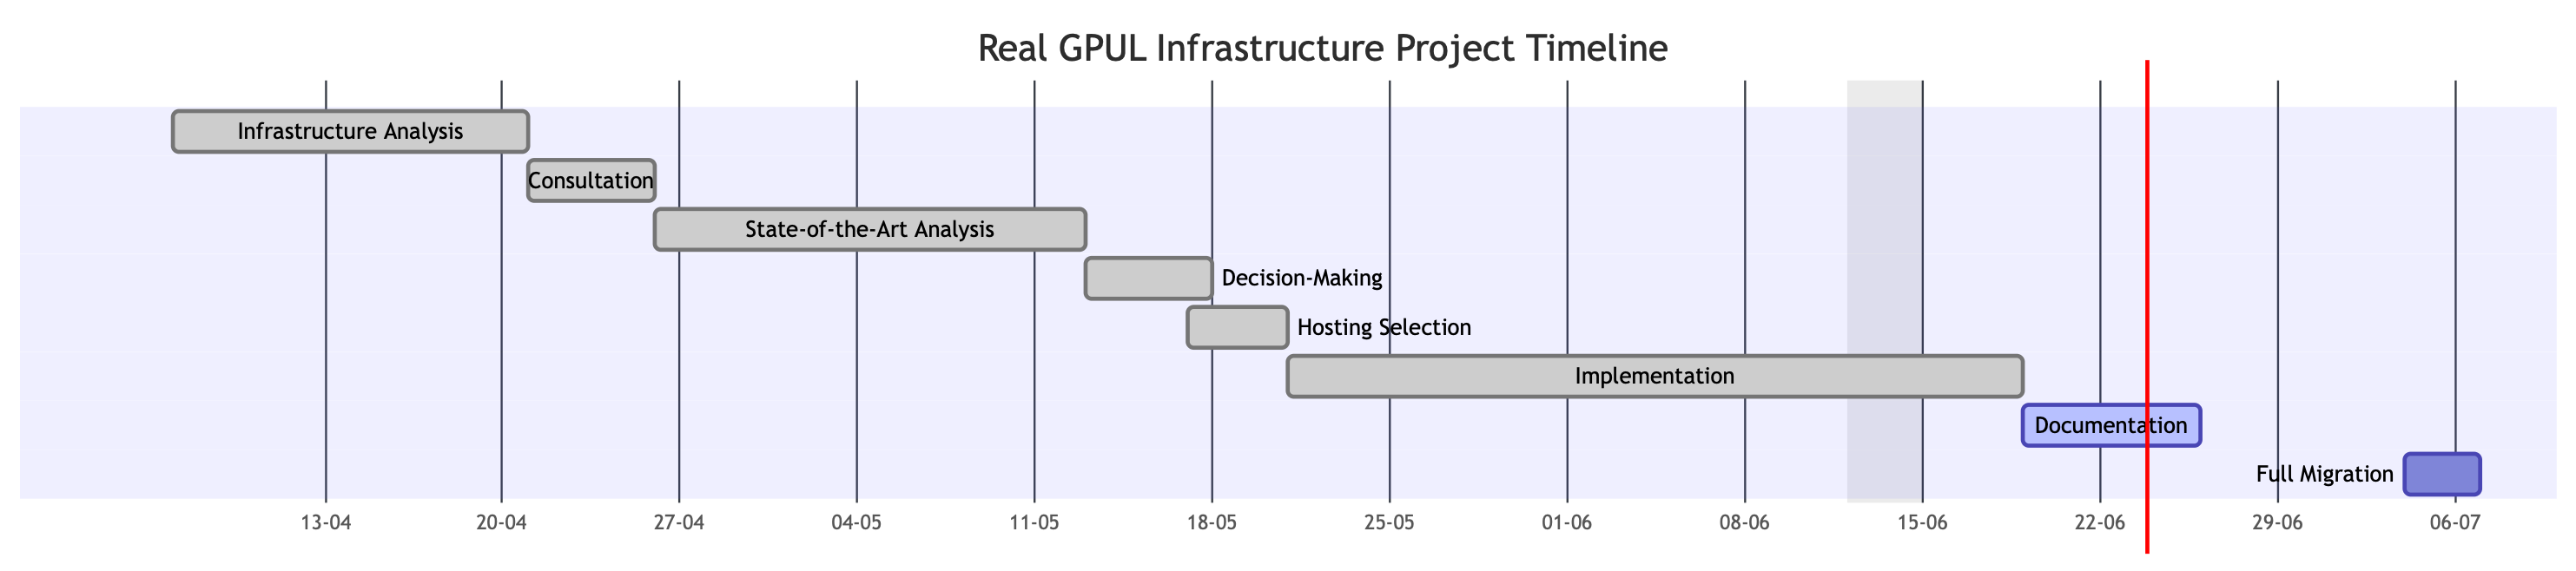
\includegraphics[width=1\textwidth]{imaxes/gantt-real.png}
  \caption{Gantt chart illustrating the real project phases.}
  \label{fig:gantt-real}
\end{figure}

\section{Cost Estimation}

Although this project was conducted under the umbrella of a volunteer-driven nonprofit organization, certain infrastructure, equipment, and labor costs can be roughly estimated to provide context on the real-world value of the work.

\subsection*{Equipment and Resources}

The development and testing work was carried out using a personal laptop and a repurposed self-hosted desktop PC:

\begin{itemize}
  \item \textbf{Laptop (development machine)}: \(\sim 1\,200€\), mid-range Linux-compatible machine.
  \item \textbf{Test server}: no acquisition cost, reused legacy hardware from prior GPUL use.
  \item \textbf{Domain name} (\texttt{gpulux.org}): \(\sim 10€\)/year.
  \item \textbf{Production server}: costs are detailed in Chapter~\ref{chap:hosting-provider}.
\end{itemize}

\subsection*{Human Resources and Labor Value}

While no direct financial compensation was involved, estimating the cost of human labor provides perspective on the real investment made, especially considering that all three individuals involved (the author and two supervisors) are not only members of the association, but also active or former board members with a high level of involvement and responsibility.

\begin{itemize}
  \item \textbf{System Administration and Infrastructure Work}: Based on the 2024 Manfred Developer Report~\cite{manfred-salary-guide}, see Figure~\ref{fig:salary-chart}, the most common salary bracket for SysAdmin roles is \textbf{€30-40K}. This work cannot be considered entry-level, as the author has over five years of professional experience and holds prior technical qualifications. Assuming a midpoint of \textbf{€35\,000} for a full-time equivalent, and with an estimated dedication of 300 hours, the work carried out corresponds to a market value of approximately \(\sim 5\,800€\).

  \item \textbf{Supervision and Guidance}: For technical supervisors involved in infrastructure or SRE roles, the most common salary bracket is higher: \textbf{€40-50K}. Using a midpoint estimate of \textbf{€45\,000} per year, their involvement (estimated 8-12 hours per supervisor) corresponds to an approximate market value of \(\sim 450€\) in total.
\end{itemize}

\begin{figure}[H]
  \centering
  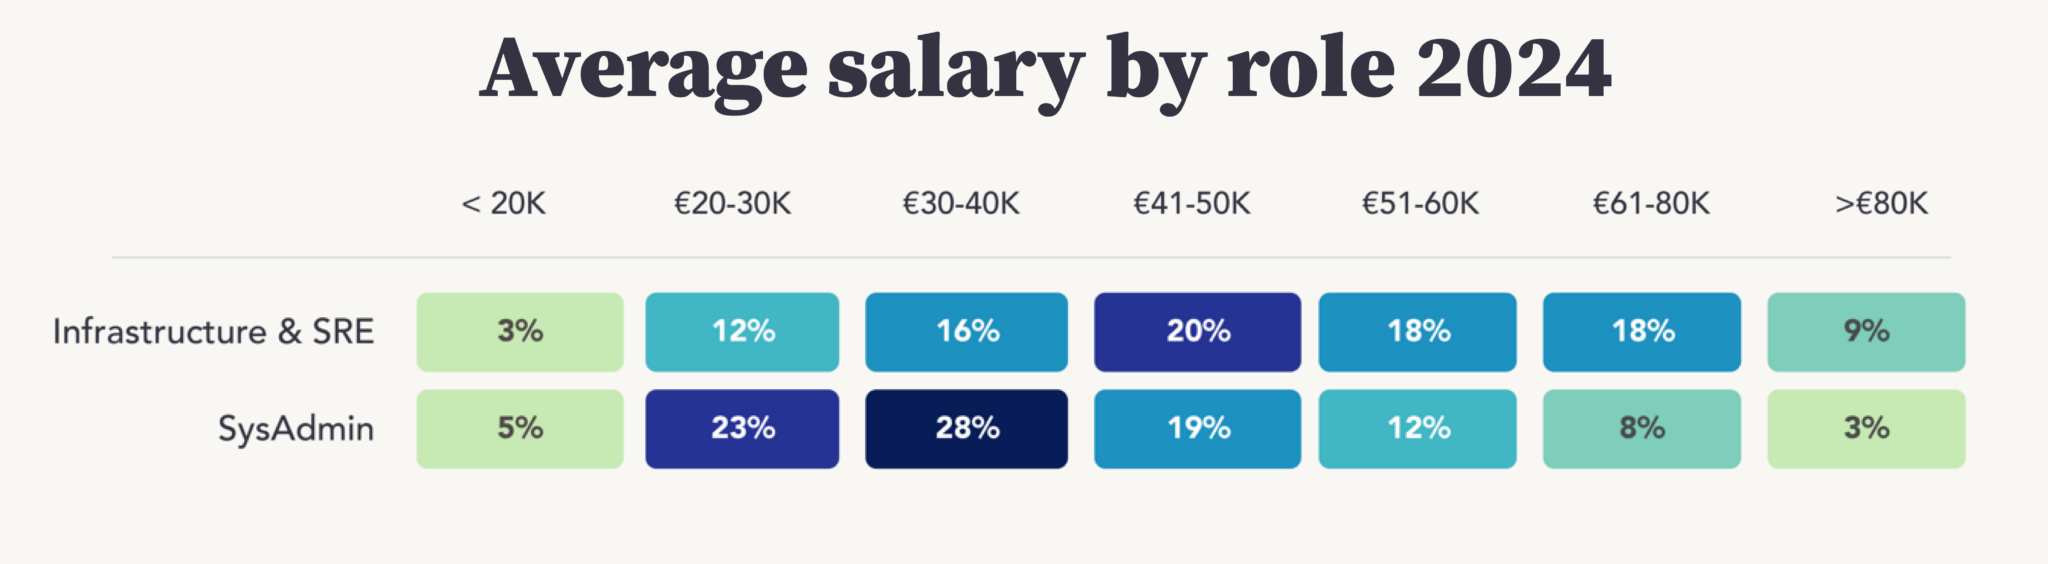
\includegraphics[width=0.8\textwidth]{imaxes/salary-chart.png}
  \caption{Average salary distribution in Spain by role.}
  \label{fig:salary-chart}
\end{figure}

These estimates illustrate that while the project was executed in a volunteer context, the real value of the technical and organizational contributions exceeds \(\sim 6\,000€\). This reinforces the importance of properly valuing community infrastructure efforts and documenting them for long-term sustainability.
